\documentclass[UTF8,zihao=-4]{ctexart}

\usepackage[a4paper,margin=2.4cm]{geometry}
\usepackage{graphicx}
\usepackage{booktabs}
\usepackage{tabularx}
\usepackage{listings}
\usepackage{fancyhdr}
\usepackage[hidelinks]{hyperref}
\usepackage{caption}

\setlength{\parindent}{2em}
\setlength{\parskip}{0.35em}
\linespread{1.28}
\pagestyle{fancy}
\setlength{\headheight}{15pt}
\fancyhf{}
\fancyhead[L]{DataLab 实验报告}
\fancyhead[R]{卓子超\quad 2025201843}
\fancyfoot[C]{\thepage}
\renewcommand{\headrulewidth}{0.4pt}
\renewcommand{\footrulewidth}{0pt}

\lstset{
  language=C,
  basicstyle=\ttfamily\small,
  columns=fullflexible,
  keepspaces=true,
  frame=single,
  framerule=0.4pt,
  numbers=none,
  breaklines=true,
  showstringspaces=false,
  aboveskip=0.6em,
  belowskip=0.6em
}

\captionsetup{font=small,labelfont=bf}

\begin{document}

\begin{center}
  {\LARGE\bfseries DataLab 实验报告}\par
  \vspace{1.2em}
  姓名\quad 卓子超\qquad 学号\quad 2025201843
\end{center}

\section{实验结果}

最终运行 \texttt{python3 test.py -V}，十二个函数全部通过，总分为 37 分。

\begin{center}
\begin{tabularx}{0.88\textwidth}{XcXc}
\toprule
函数 & 得分 & 函数 & 得分 \\
\midrule
bitAnd & 1/1 & bitXor & 1/1 \\
samesign & 2/2 & logtwo & 4/4 \\
byteSwap & 4/4 & reverse & 3/3 \\
logicalShift & 3/3 & leftBitCount & 4/4 \\
float\_i2f & 4/4 & floatScale2 & 4/4 \\
float64\_f2i & 3/3 & floatPower2 & 4/4 \\
\bottomrule
\end{tabularx}
\end{center}

\begin{figure}[htbp]
  \centering
  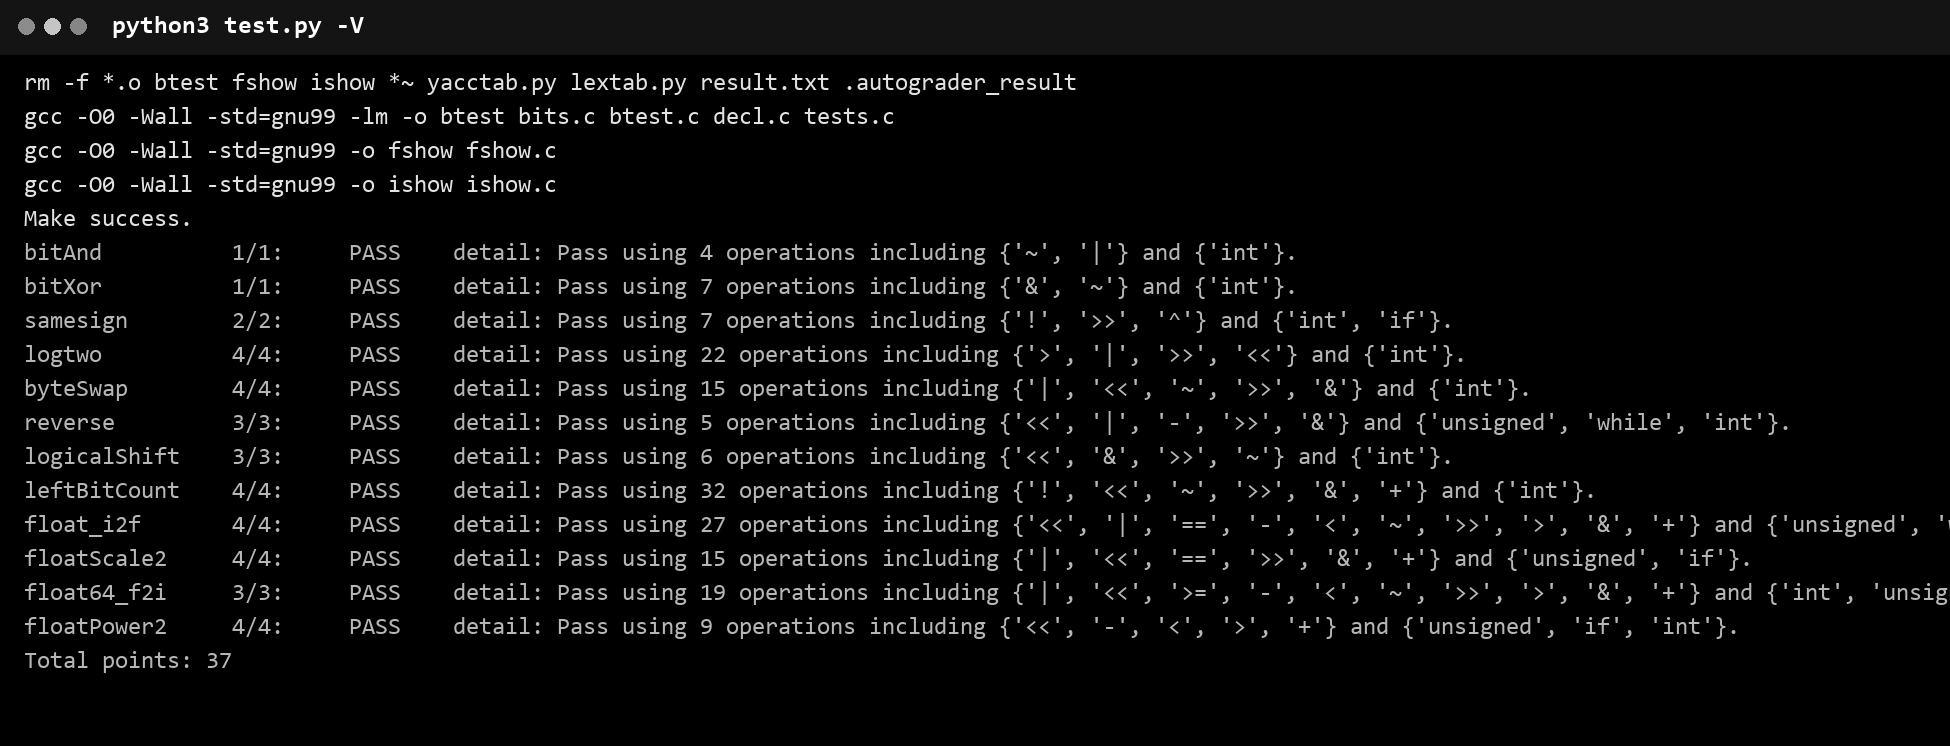
\includegraphics[width=\textwidth]{imgs/test-results-bw.png}
  \caption{完整测试结果}
\end{figure}

\section{解题记录}

\subsection{几个基础位运算}

\texttt{bitAnd} 和 \texttt{bitXor} 主要用到了德摩根律。前者把按位与改写为

\begin{lstlisting}
~(~x | ~y)
\end{lstlisting}

后者分别排除两个输入同时为 1 和同时为 0 的位置。\texttt{samesign} 需要额外处理零，因为题目规定零既不是正数也不是负数。两个参数都非零时，再比较右移 31 位后的符号。

\subsection{logtwo}

这个函数要找最高位 1 的位置。我没有逐位循环，而是按 16、8、4、2、1 位分段判断。以第一次判断为例，\texttt{v >> 16} 非零时，最高位一定在高 16 位中，于是记录 16，并把已经确定的部分移走。

\begin{lstlisting}
shift = ((v >> 16) > 0) << 4;
result = shift;
v = v >> shift;
\end{lstlisting}

后面几轮保持相同结构。各轮得到的值分别占据结果中的不同二进制位，因此可以用按位或合并。

\subsection{byteSwap 和 reverse}

我开始写 \texttt{byteSwap} 时，直接使用了 \texttt{x >> n}。后来检查示例才发现，\texttt{n} 和 \texttt{m} 表示字节编号，一个字节对应 8 位，所以应先写成

\begin{lstlisting}
n = n << 3;
m = m << 3;
\end{lstlisting}

接着用 \texttt{0xFF} 取出两个字节，清空原位置，再交换写回。

\texttt{reverse} 的第一版把最低位重新放回了 \texttt{v} 的最高位，那样得到的是循环移位。我后来增加了单独的 \texttt{result}，每次把旧结果左移一位，再接上 \texttt{v} 的最低位。

\begin{lstlisting}
result = (v & 1) | (result << 1);
v = v >> 1;
\end{lstlisting}

循环次数要取 32，而且条件应写成 \texttt{while (times)}。若写成 \texttt{while (!times)}，初值为 32 时循环一次也不会执行。

\subsection{logicalShift 和 leftBitCount}

\texttt{logicalShift} 的困难在于有符号数右移会补符号位。我的处理是先完成算术右移，再生成一个高 \texttt{n} 位为 0 的掩码，把补进来的 1 清掉。

\begin{lstlisting}
(x >> n) & ~(((1 << 31) >> n) << 1)
\end{lstlisting}

这里不能直接用 \texttt{0x80000000 >> n} 代替前半段。这个常量通常会按无符号数处理，右移时左边补 0，无法生成连续的高位掩码。

\texttt{leftBitCount} 也使用了分段判断。表达式 \verb|!~(x >> 16)| 用来检查最高 16 位是否全为 1。判断成立后，把计数增加 16，并左移掉已经统计的部分，然后继续检查 8、4、2、1 位。最后再检查一次剩余最高位，才能让输入为 \texttt{-1} 时得到 32。

\subsection{float\_i2f}

整数转 Float32 时，我先把符号和绝对值分开，再寻找绝对值的最高位 1。这个位置决定真实指数，存储指数还要加上偏置 127。

有效位不超过 24 位时，左移对齐即可。有效位更多时，需要丢掉低位。我记录被丢弃部分，并按就近舍入到偶数处理。丢弃部分超过一半时进位；恰好等于一半时，只在保留部分最低位为 1 时进位。最后把舍入值加到已经组合好的位模式上，尾数全为 1 时，进位会直接进入指数域。

\subsection{另外三个浮点函数}

\texttt{floatScale2} 按指数分类。指数为 0 时把尾数左移一位，跨过非规格化边界时会自然进入指数域；普通规格化数把指数加一；指数为 \texttt{0xFE} 时返回同符号的无穷；NaN 和无穷保持原位模式。

\texttt{float64\_f2i} 的输入被拆成高低两个 32 位参数。我从高半部分取出符号、11 位指数和尾数高 20 位，再补回规格化数隐含的 1。真实指数较小时，整数部分完全来自高半部分；指数较大时，再从 \texttt{uf1} 的高位补入需要的位。右移会直接丢弃小数部分，所以满足向零舍入。

\texttt{floatPower2} 只需要处理指数范围。小于 $-149$ 时返回 0，$[-149,-127]$ 落在非规格化区间，$[-126,127]$ 使用偏置指数，超过 127 时返回正无穷。

\section{总结}

这次实验中，最容易出错的地方是把字节编号当成位数、把循环移位当成位反转，以及忽略浮点舍入。逐项查看失败样例比只检查几个普通输入更有效。最终版本通过全部测试，整数函数的运算符数量和浮点函数的边界处理也符合题目限制。

\section{参考资料}

\begin{enumerate}
  \item Randal E. Bryant、David R. O'Hallaron：《深入理解计算机系统》
  \item 课程课件中关于位运算的内容
\end{enumerate}

\end{document}
